\chapter{Introduction} 
% \addcontentsline{toc}{chapter}{Introduction}

    \section{Motivation}
        I chose this thesis project because of my extended knowledge around the subject and because i thought i could combine all of my past research into this.

        Before i even started writing, i already had experience working in the following fields and i will briefly present my computer science background

        \subsection{Background}
            The following sections highlight pieces of my work that are relevant to this thesis. Each included project is significant due to specific implementations that are directly or indirectly connected to this paper.

            \subsubsection{Computer Graphics Experience}
                \begin{SCfigure}[0.9][h] 
                    \caption{Fractal Tree Visualization
                    
                    (usage of p5.js primitive functions in a recursive manner)

                    \href{https://www.youtube.com/watch?v=ajd0GGZgnDg&list=PL-j3UE1st04BZqRXq6eUBHpovhKjA1kiX&index=7}{showcase}}
                    
                    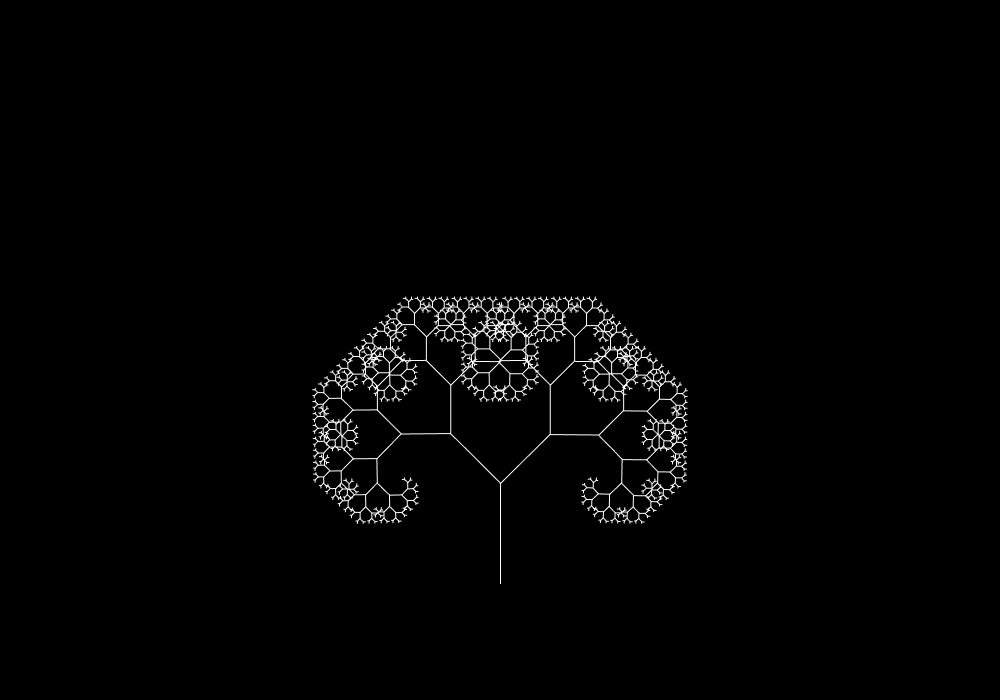
\includegraphics[width=8cm]{fractal.png}
                    \centering
                \end{SCfigure}                    
                \begin{itemize} 
                    \item Supershape Rendering Techniques 
                    \item Function Visualizer in OpenGL 
                    \item Complex Function Visualizer 
                \end{itemize}

            \subsubsection{Game Development Experience} 
                \begin{itemize} 
                    \item 3D Open World Environment Development 
                    \item Studies of Vector Movements in Unity 
                \end{itemize}

                % \subsubsection{in computer graphics}
            %     \subsubsection{fractal tree}
            %     \subsubsection{supershapes}
            %     \subsubsection{visualising basic function in opengl}
            %     \subsubsection{moving towards complex functions (mandelbrot series, julia fatou series)}
            %     \subsubsection{3D rendering}

            \subsubsection{in game development}
                my game development studies had mostly been around 3D open-world games. Being fascinated by rockstar's grand theft auto series i want to build something similar. i always wondered how cj was able to move in all the directions and calculating how there would be way too many paths to generate all the possible outcomes. so there should be smarter ways to do movement.
                And there is. Using vectors.
                My unity projects were mostly about perfectioning the 3D vector movement. Something that i also tried to implement in the opengl framework.   

        \subsection{Goal}
            I challenged myself to dig deeper into Game Development. I wanted to understand what makes all the pretty images move. i already had somewhat of an understanding of how the frames have to be processed independently and displayed in a fastly manner in order to trick the brain. but i wanted to go deeper then that.

            i already understood how to do certain simple tasks in unity, but i was so fascinated of the "transform.position = Vector2.One * scalar" command that i wanted to create a similar environment. 




            the intention of this project is to act as a foundation for a possible game engine that i will continue to deveop in the future. 

            a game engine is no easy task, there are many running parts and each of them must be SOLID. 

        % \subsection{Progress}

        %     until now i have the opengl framework in a stable state, this journey gave me a deeper understanding of all the running parts needed. 

        %     Now that i've been able to replicate some of the foundational concepts in enclosed environments, in the future i tend to use some already existing frameworks for physics and scene management and also ml libraries like scipy.

    \section{Literature Review}
            
            in order to achieve this project i have went through multiple pieces of literature.

            the ones i used most extensively are:
                \subsection{Books}
                    \subsubsection{OpenGL SuperBible}
                        SuperBible provided a thorough introduction to OpenGL,
                        detailing its functions and capabilities. This resource
                        was instrumental in understanding the core principles of
                        rendering and shading, which are fundamental to the
                        development of any graphics application. By following
                        the examples and exercises in this book, I was able to
                        implement efficient rendering pipelines and gain a deep
                        understanding of shader programming.
                    \subsubsection{Computer Graphics (Donald Hearn)}
                        % this gave me an in-depth understanding of the computer graphics field and also very insightful insides to primitives, drawing algorithms, popular solutions to popular problems. 
                        Donald Hearn's Computer Graphics offered a comprehensive overview of graphics
                        primitives and the algorithms used to draw them. The book's clear explanations
                        of line drawing algorithms, polygon filling techniques, and transformations were
                        particularly beneficial. Implementing these algorithms in my application allowed
                        me to create accurate and efficient rendering routines.
                    \subsubsection{Mathematics for Game Development (Christopher Tremblay)}
                        % i held this book very closely while writing the math engine for the game-engine.
                        % i recaped my veVctorial knowledge and understood which operators are most relevant in such projects and why. 
                        Christopher Tremblay's book on
                        mathematics for game development provided a solid
                        foundation in vectorial math, which is crucial for tasks
                        such as collision detection and physics simulation. The
                        detailed explanations of vector operations, matrix
                        transformations, and geometric algorithms were directly
                        applied in the development of the vector math library in
                        my application.
                    \subsubsection{C++ (Bjarne Stroustrup)}
                        Bjarne Stroustrup's definitive
                        guide to C++ significantly improved my programming
                        skills, enabling me to write efficient, robust, and
                        maintainable code. The book's coverage of advanced C++
                        features, such as templates, polymorphism, and the
                        Standard Template Library (STL), was particularly
                        valuable in structuring my application and optimizing:want
                        performance.
                \subsection{Papers}
                    \subsubsection{ml agents that can communicate to one another}
                    \subsubsection{comp graphics projects from stanford}
                    \subsubsection{...}

    \section{Theorethical overview}
        \subsection{Electronics}
        \subsection{Math}
        \subsection{Computer Graphics}
        \subsection{Game Development}
        \subsection{Coding Practices}


% The first ever game created was 'Tennis for Two' and was played on an oscilloscope. From then, gaming evolved from simple pixelated experiences to complex, immersive digital worlds.

% "Before game engines, games were typically written as singular entities: a game for the Atari 2600, for example, had to be designed from the bottom up to make optimal use of the display hardware (...) 
% Even on more accommodating platforms, very little could be reused between games."

% (Game Engine, Wikipedia)

% % (Did u know that the first Roller Coaster Tycoon was written completly in Assembly?)

% Programmers needed a way to make the game building process more efficient. So around the mid-1990s, thanks to Epic Games and their launch of the Unreal Engine and thanks to Id Software's Doom and Quake games the term "Game Engine" started to become more and more popular.

% Fast forward mid-2020s, now we have access to ultra realistic tank simulators for soldier training ( projectName ), surreal worlds filled with fantasy creatures ( Middle Earth: Shadow Of Mordor ) and even indie projects like Hyerbolica that portraits how a non-euclidian world would behave like. Projects like these would've been way harder ( if not actually impossible ) to pull off without the help of game engines.

% \pagebreak

% \section{Game Engines}
% "The line between a game and its engine is often blurry. Some engines make a reasonably clear distinction, while others make almost no attempt to separate the two. ( ... ) We should probably reserve the term
% 'game engine' for software that is extensible and can be used as the foundation for many different games without major modification."

% ( Game Engine Architecture. by Jason Gregory )

% \begin{figure}[!h]
%     \centering
%     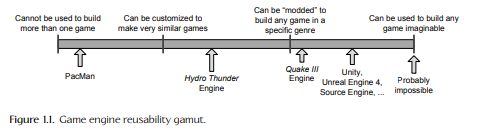
\includegraphics[width=1\linewidth]{chapters/gameEngine Usability.png}
%     \caption{Game Engine Reusability Gamut}
%     \label{fig:Game-Engine Reusability}
% \end{figure}



% Behind the curtains of any interactive application there is most likely a Game Engine. 
% You have probably heard before about Unity and Unreal but there are many more game engines out there. Some of them are In-House, some of them are Open-Source, some of them are made for a specific Genre. But none of them is offering Built-In Machine Learning Integration. 

% \subsection{What does a Game Engine offer?}

% While not limited to, some of the tools we expect a game engine to offer are: 
% \begin{enumerate}
%     \item Input Handling
%     \item Player Mechanics
%     \item Game-Specific Rendering
%     \item Collision \& Physics
%     \item Audio Playback
%     \item Game Cameras
%     \item Ai \& Behaviour Management
%     \item Online Multiplayer
%     \item Scene Graph
%     \item Scripting System
%     \item Visual Effects
% \end{enumerate}

% \section{What is Machine Learning?}

% \begin{enumerate}
%     \item predicts text, predicts what the next word in a sentence would most likely be.
%     \item it's too broad of a topic to be able to explain in detail in just one paper. And it's also not the purpose of this paper. This paper only wants to use the power of ai to simulate better npc's in games.
%     \item for the purpose of this, i will not try to recreate or train an machine learning model, i will use an already existing one: GPT 3.5-Turbo by OpenAI.
% \end{enumerate}

% \subsection{Machine Learning in Game Engines}
% \begin{enumerate}
%     \item Inworld Origins are already working on a solution for implementing GPT4 to be used in a NPC dialogue scenario.
%     \item There is this study where multiple GPT4 agents that can simulate believable human behavior. (Generative Agents: Interactive Simulacra of Human Behavior)
%     % https://arxiv.org/pdf/2304.03442.pdf
%     \item Currently, there are no game engines that have Machine Learning Systems built-in. 
% \end{enumerate}

% \section{Scope and Objectives of the Thesis}
% \begin{enumerate}
%     \item exploration, development, and evaluation of a game engine that integrates GPT-based machine learning capabilities 
%     \item explore the architecture of a game engine while building a basic one in Python using OpenGL.
%     \item explore what it means to add machine learning capabilities to a game engine. 
%     \item The focus of this research is on leveraging the power of natural language processing (NLP) and GPT models to enhance various aspects of game development, including storytelling, character interactions, procedural content generation, and player experiences.
% \end{enumerate}

